\section{Interaction}\label{sec:interact}

We shall illustrate \UTP2's use by walking through a simple proof,
from a theory of sets, regarding the commutativity of set intersection.

\noindent
We start by launching the theorem prover, and we assume that some theories have been
preloaded: \texttt{Sets}%
\footnote{The \texttt{\$0} suffix is a version number}%
, \texttt{Equality}, \texttt{Logic} and \texttt{\_ROOT} (a base theory always present).
All theories have access to definitions and laws from lower theories.


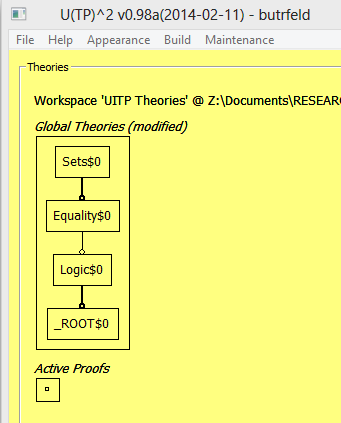
\includegraphics[scale=0.5]{01-initial-state.png}

\noindent
If we double-click on the \texttt{Sets} box,
a window opens up showing the ``Laws'' of the Set theory.
Laws have names, a ``provenance'' indicator, side-conditioning,
and their defining schema (a predicate).

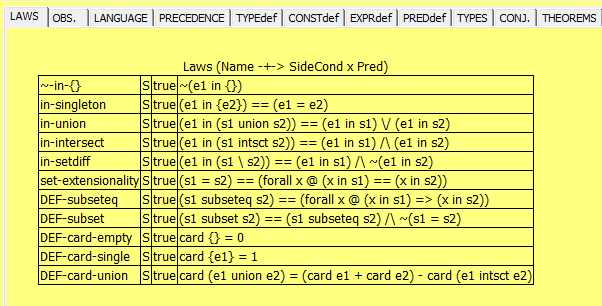
\includegraphics[scale=0.5]{02-set-axioms.png}

\noindent
Clicking on the ``CONJ.'' tab shows some conveniently preloaded conjectures,
which have yet to be proven.

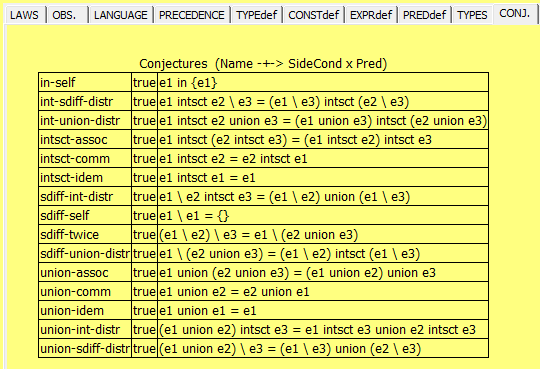
\includegraphics[scale=0.5]{03-set-conjectures.png}

\noindent
Double-clicking on the \texttt{intsct-comm} row (5th) opens up a proof window,
and we use its setup menu to select the ``Reduce'' strategy,
which attempts to transform the goal predicate into TRUE.
Other strategies, depending on the goal structure include: ``left-to-right'',
for equality/equivalence conjectures, that
converts the lefthand side until equal to the righthand side,
or ``reduce-both'' which tries to transform both sides into some common form.

In the proof window we have the goal and side-conditions displayed,
and there is some material about heuristics we ignore in this paper.
The lower half of the proof window displays the ``TARGET'',
determined by the goal and the chosen strategy.
Some context information is also shown, the most important being the free variables,
and the type, in this case, of each side of the equality.
We see the starting goal at the bottom, in bold and underlined%
\footnote{The ``Matches'' subwindow will not be discussed here}%
:

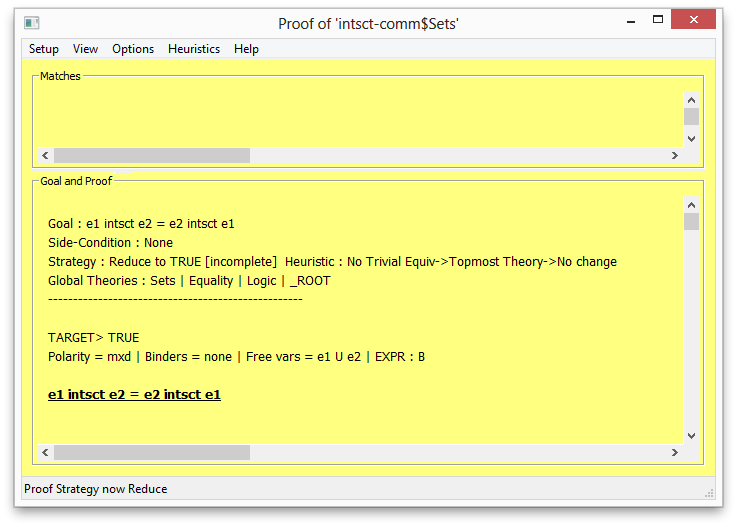
\includegraphics[scale=0.5]{06-starting-REDUCE-proof.png}

\noindent
If we right-click anywhere in the ``Goal and Proof'' subwindow,
then a menu of laws applicable to the goal pops-up.
In effect the goal was matched against all the laws present in the
\texttt{Sets}, \texttt{Equality}, \texttt{Logic} and \texttt{\_ROOT} theories, the successful matches were then ranked
(by various user-selectable heuristics), the top twenty chosen, then applied to the
goal to show the result, and presented in the menu.

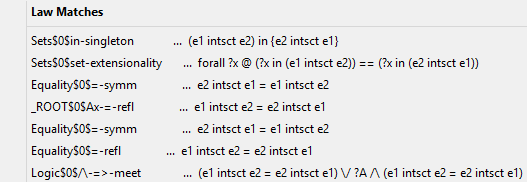
\includegraphics[scale=0.5]{07-laws-applicable-to-goal.png}

\noindent
If we pick the second, ``set-extensionality'', as it has new variables not present in the goal, (e.g. \texttt{?x}), we are asked to supply instances for these, with a reasonable default being offered.
This feature is not obviously useful in this example (except if \texttt{x} was present elsewhere) but comes in handy when matching the rhs of a law like $A \lor (A \land B) \equiv A$, to get the rhs,
in which we are free to instantiate $B$ as we see fit.

  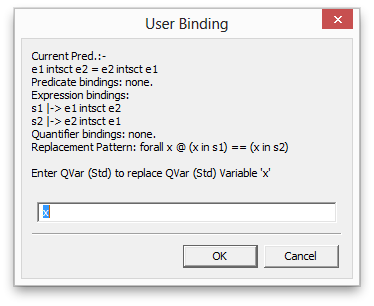
\includegraphics[scale=0.5]{08-instantiating-qvars.png}

\noindent
If we go with the default suggestion, then we obtain the following proof state:

  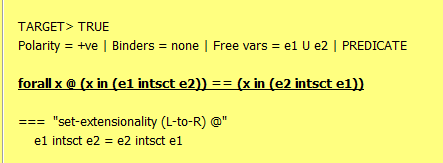
\includegraphics[scale=0.5]{09-extensionality-applied.png}

\noindent
We can use arrow-keys to move around the goal, changing the proof ``focus''.
If we go ``down'' twice, we focus in on the first set membership assertion.
It is worth noting that the line above records that the focus is on an expression (EXPR)
of type boolean (\texttt{B}). \UTP2\ has a on-the-fly type inference algorithm that runs
every time the focus changes%
\footnote{speed has never been a problem with this}%
, and is used by the law matching algorithm to avoid spurious matches.
We avoid lots of explicit type annotations, preferring to deal with such issues
behind the scenes. This is of course in keeping with the general traditional UTP approach
to theorem development.

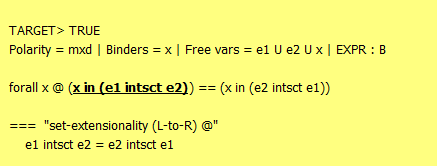
\includegraphics[scale=0.5]{11-moving-down-again.png}

\noindent
Right-clicking now leads to laws relevant to the focus:

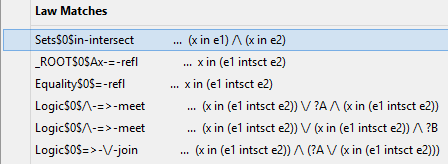
\includegraphics[scale=0.5]{12-laws-applicable-to-focus.png}

\noindent
If we pick the first option, then we get a conjunction of simpler membership statements.

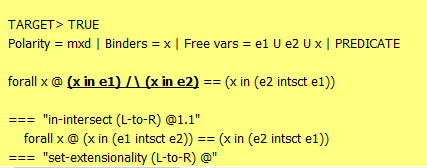
\includegraphics[scale=0.5]{13-intersect-axiom-applied.png}

\noindent
Moving to the righthand side of the equality, we can apply the same \texttt{in-intersect} law,
then apply the commutativity of conjunction, pull back out and we get
instances of the reflexivity of equals. Finally we get rid of a vacuous quantifier,
so resulting in the goal \texttt{TRUE}, and \UTP2\ proclaims!

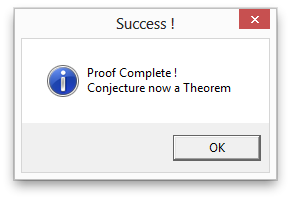
\includegraphics[scale=0.5]{17-proof-complete.png}

\noindent
Examining the ``THEOREMS'' tab in the Set theory window shows our new theorem.

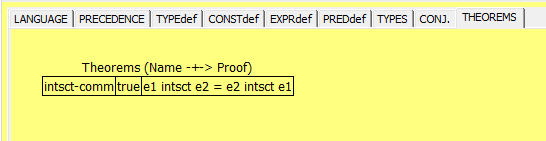
\includegraphics[scale=0.5]{20-our-new-theorem.png}

\noindent
Right-clicking on it gives another pop-up menu of interesting things to do with it.

  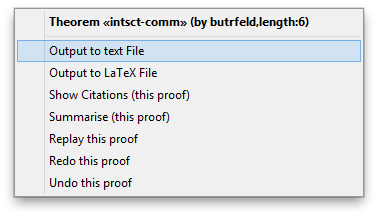
\includegraphics[scale=0.5]{21-saving-text-version.png}

\noindent
We render a simple text version of the resulting proof:
\begin{verbatim}
Complete Proof for 'Sets$intsct-comm
Goal : e1 intsct e2 = e2 intsct e1
Strategy: Reduce to TRUE

     e1 intsct e2 = e2 intsct e1
 ===   " set-extensionality (L-to-R) @ "
     forall x @ (x in (e1 intsct e2)) == (x in (e2 intsct e1))
 ===   " in-intersect (L-to-R) @1.1 "
     forall x @ (x in e1) /\ (x in e2) == (x in (e2 intsct e1))
 ===   " in-intersect (L-to-R) @1.2 "
     forall x @ (x in e1) /\ (x in e2) == (x in e2) /\ (x in e1)
 ===   " /\-comm (R-to-L) @1.2 "
     forall x @ (x in e1) /\ (x in e2) == (x in e1) /\ (x in e2)
 ===   " Ax-==-id (R-to-L) @1 "
     forall x @ TRUE
 ===   " forall-vac (L-to-R) @ "
     TRUE
\end{verbatim}

\noindent
We have only skimmed over the interactive proof features of \UTP2 here.
Others include
\begin{itemize}
  \item keyboard shortcuts to apply built-in procedures to the focus,
    e.g., convert to disjunctive normal form
  \item
    a clickable help feature in the proof window
  \item strategies to support inductive proofs
  \item
    all tables in each tab of each theory can be edited, with entries added
    or deleted --- even laws!
  \item
    Some of the tabs, (``OBS.'',``LANGUAGE'',``PRECEDENCE'') have
    tables that support user definitions of languages.
    See \cite{conf/utp/Butterfield12} for further details.
\end{itemize}
